\documentclass[a4paper]{scrartcl}

\usepackage[utf8]{inputenc}
\usepackage[ngerman]{babel}
\usepackage[T1]{fontenc}
\usepackage{amssymb}
\usepackage{mathtools}
\usepackage{gensymb}

\usepackage{graphicx}

\usepackage{geometry}
\geometry{verbose,a4paper,tmargin=25mm,
bmargin=25mm,lmargin=25mm,rmargin=25mm}

\usepackage{float}
\usepackage{enumitem}
\setlist{nosep} % or \setlist{noitemsep} to leave space around whole list
\setlength\parindent{0pt}
\usepackage{hyperref}
\hypersetup{
    colorlinks,
    citecolor=black,
    filecolor=black,
    linkcolor=black,
    urlcolor=black
}


\title{Battletanks - Benutzerhandbuch}
\subtitle{Universität Würzburg Informatik Softwarepraktikum Wintersemester 2016/17}
\author{Armin Bernstetter, Stefan Ernst, Nicolas Fella}

\begin{document}

\maketitle
\tableofcontents
\newpage

\section{Allgemeine Programmbeschreibung}
'Battletanks' ist ein lokales, Desktop-basiertes Multiplayerspiel. Es wurde im Rahmen des Softwarepraktikums Informatik der Universität Würzburg im Wintersemester 2016/17 entwickelt.

In diesem Spiel können bis zu vier Spieler mit je einer Spielfigur auf einem Top Down 2D Spielfeld gegeneinander antreten, indem sie gegnerische Spielfiguren abschießen bis die benutzerdefinierte Spielzeit verstrichen ist. Der Gewinner ist am Ende des Spiels der Spieler mit den meisten Abschüssen sowie den wenigsten Toden.
Alle Spieler benutzen zur Bedienung des Spiels gemeinsam eine Tastatur mit unterschiedlicher Tastenbelegung je Spieler. Jede der Spielfiguren besitzt unterschiedliche Statuswerte für Lebenspunkte, Schaden, Schadensreduktion und Schussfrequenz.
Das Spielfeld kann manuell aus einer externen Datei eingelesen werden.



\section{Erste Schritte}
Um 'Battletanks' zu spielen benötigen Sie nur einen beliebigen Computer mit einem Mac, Linux oder Windows-Betriebssystem sowie die aktuelle Java SE Runtime Environment (JRE) 8. Diese können Sie beispielsweise \href{http://www.oracle.com/technetwork/java/javase/downloads/jre8-downloads-2133155.html}{\textbf{\textit{hier}}} auf der Seite von Oracle herunterladen.

Das Programm selbst wird als eine ausführbare .jar-Datei ausgeliefert, Sie müssen es also nicht erst installieren sondern können das Spiel sofort starten falls Sie eine JRE installiert haben.

\newpage
\section{Benutzung}
\subsection{Menü}

\begin{figure}[H]
  \textbf{Screenshot Menü:}\par\medskip
  \centering
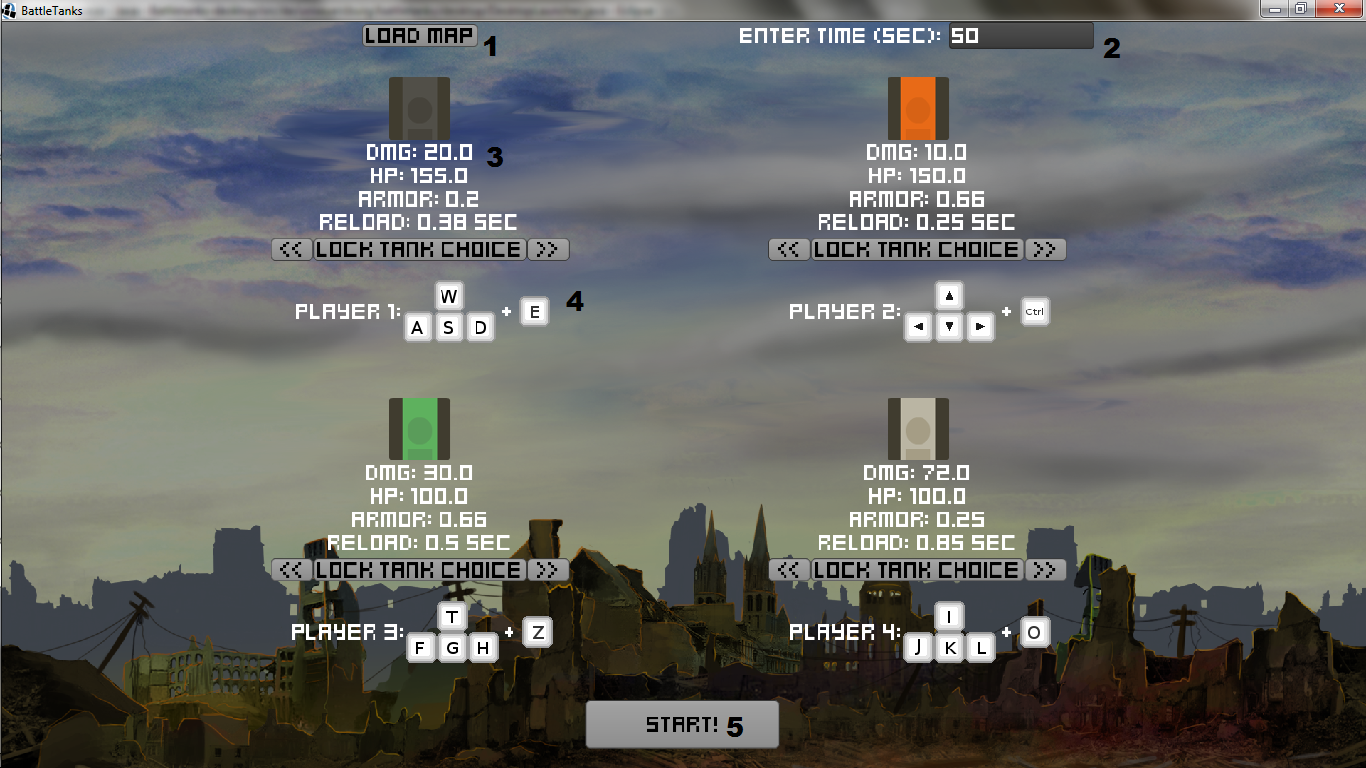
\includegraphics[width=15cm]{screenshot_menu.png}
\caption{1: Map Laden, 2: Zeit Eingeben, 3: Spielfigur auswählen, 4: Tastenbelegung des jew. Spielers,
5: Spiel starten}
\end{figure}



\subsubsection{Eine Map laden}
\begin{figure}[H]
  \textbf{Screenshot FileChooser:}\par\medskip
  \centering
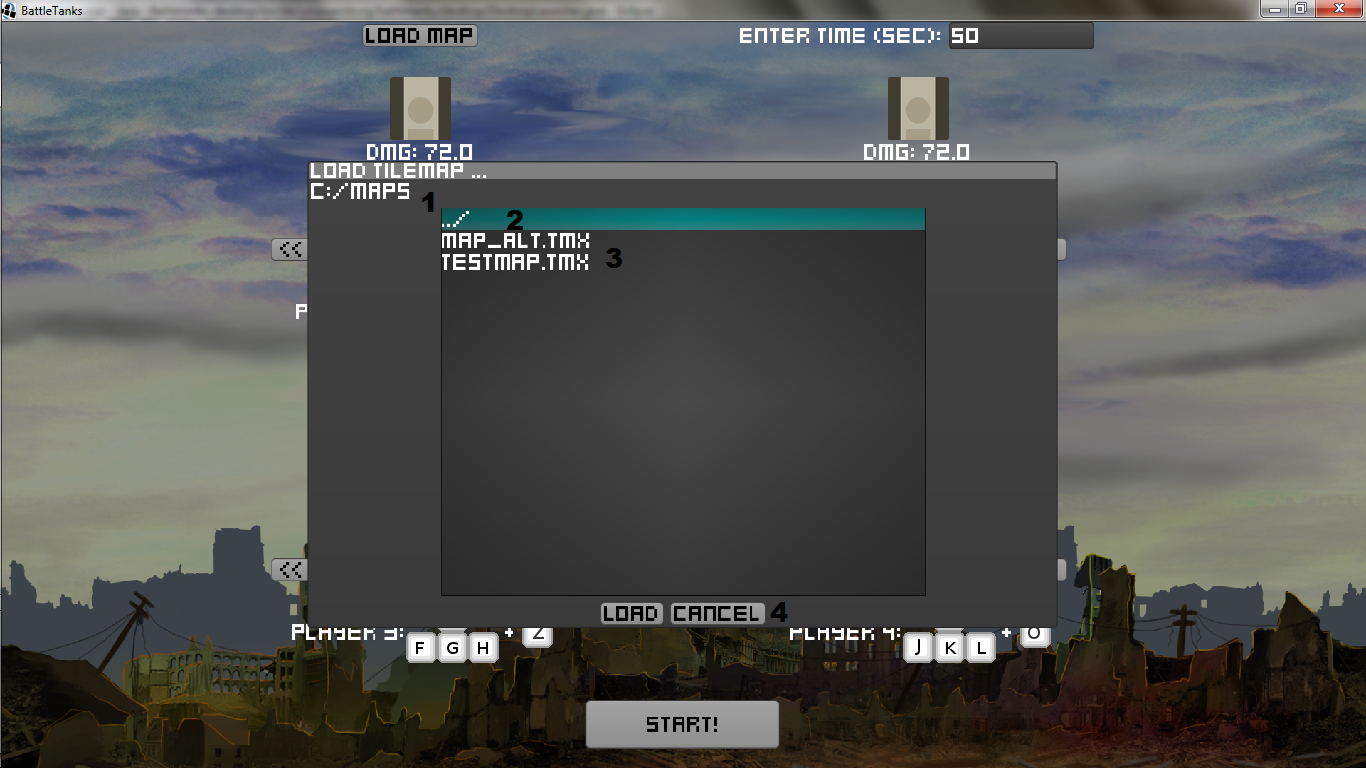
\includegraphics[width=15cm]{screenshot_filechooser.png}  
\caption{1: Anzeige des aktuellen Ordnerpfades, 2: Wechseln in den vorherigen Ordner, 3: Die zur Auswahl stehenden Maps, 4: Ausgewählte Map laden oder Abbrechen}
\end{figure}
 
Laden Sie eine Map, indem sie den 'Load Map'-Button drücken (Abbildung 1: 1) und eine der mitgelieferten Maps im angezeigten Ordner laden (Abbildung 2). Diese Maps wurden so erstellt, dass Sie auf ihnen spielen können. Falls Sie keine Map manuell laden wollen, wird das Spiel auf der Standardmap stattfinden.


Alternativ können Sie zu einem eigenen Verzeichnis navigieren und eine andere Map laden. Diese muss im .tmx Dateiformat vorliegen und kann zum Beispiel mit dem Mapeditor Tiled (\url{http://www.mapeditor.org/}) erstellt werden. 

Die Spielfiguren starten in je einer der vier Spielfeldecken, weshalb diese in den mitgelieferten Maps freigehalten werden. Falls Sie eine Map laden, die nicht diesen Anforderungen entspricht kann es zu Komplikationen im Spielverlauf kommen.
\subparagraph{Spawnpunkte:}
\begin{itemize}
\item Player 1: Links Oben
\item Player 2: Rechts Oben
\item Player 3: Links Unten
\item Player 4: Rechts Unten
\end{itemize}

\subsubsection{Spielzeit eingeben}
Geben Sie die gewünschte Spielzeit in Sekunden ein. (Abbildung 1: 2) Falls Sie keine eigene Zeit eingeben startet das Spiel mit dem Defaultwert von 50 Sekunden. 

\subsubsection{Tastenbelegung}
Sie können aus vier verschiedenen Tastenbelegungen auswählen, die im Menü angezeigt werden (Abbildung 1: 4). Jede Tastenbelegung kann nur von einem Spieler benutzt werden. Vier Tasten dienen der Bewegung, mit der weiteren Taste können Sie schießen. 
Beispielsweise besitzt Player 1 die Bewegungstasten WASD für Oben, Links, Unten, Rechts und die Taste E für das Feuern der Waffe.

\newpage
\subsubsection{Die Spielfiguren}
Wählen Sie aus einer von fünf verschiedenen Spielfiguren aus, indem Sie mit den Pfeil-Buttons durch die verfügbaren Panzer wechseln.(Abbildung 1: 3) 

Diese besitzen verschiedene Werte für Schaden, Leben, Schussfrequenz/Nachladezeit und Schadensreduktion/Rüstung, welche im Menü angezeigt werden. Manche Panzer besitzen hohe Schadenswerte, dafür aber nur geringe Lebenspunkte, bei anderen ist es umgekehrt. Richten Sie sich bei der Entscheidung nach eigenen Vorlieben sowie nach ihren Mitspielern um möglicherweise deren Auswahl zu kontern.


Wenn Sie sich für eine Figur entschieden haben, drücken Sie den 'Lock Tank Choice'-Button, um festzulegen mit welchem Panzer Sie spielen wollen.



\begin{tabular}{|c|c|}
\hline 
\textbf{Panzer} & \textbf{Daten} \\ 
\hline 

\includegraphics[width=1.5cm]{tankBeige.png} & 
\parbox[c]{5cm}{Damage: 72 \\ HP: 100 \\ Armor: 0.25 \\ Reload: 0.85 sec\\}
\\ 
\hline 

\includegraphics[width=1.5cm]{tankBlack.png} & \parbox[c]{5cm}{Damage: 20 \\HP: 155 \\  Armor: 0.2 \\ Reload: 0.38 sec\\} \\ 
\hline 

\includegraphics[width=1.5cm]{tankBlue.png} & \parbox[c]{5cm}{Damage: 20\\HP: 179 \\  Armor: 0.4\\ Reload: 0.5 sec\\} \\ 
\hline 

\includegraphics[width=1.5cm]{tankGreen.png} & \parbox[c]{5cm}{Damage: 30\\HP: 100\\  Armor: 0.66\\ Reload: 0.5 sec\\} \\ 
\hline 

\includegraphics[width=1.5cm]{tankRed.png} & \parbox[c]{5cm}{Damage: 10\\HP: 150\\  Armor: 0.66\\ Reload: 0.25 sec\\} \\ 
\hline 
\end{tabular} 

\subsubsection{Starten des Spiels}
Drücken Sie auf den 'START!'-Button (Abbildung 1: 5). Falls Sie keine oder eine ungültige Zeit eingegeben oder keine Spielfigur ausgewählt haben erscheint eine Fehlermeldung.

\newpage
\subsection{Bedienung des Spiels}
\begin{figure}[H]
  \textbf{Screenshot Game:}\par\medskip
  \centering
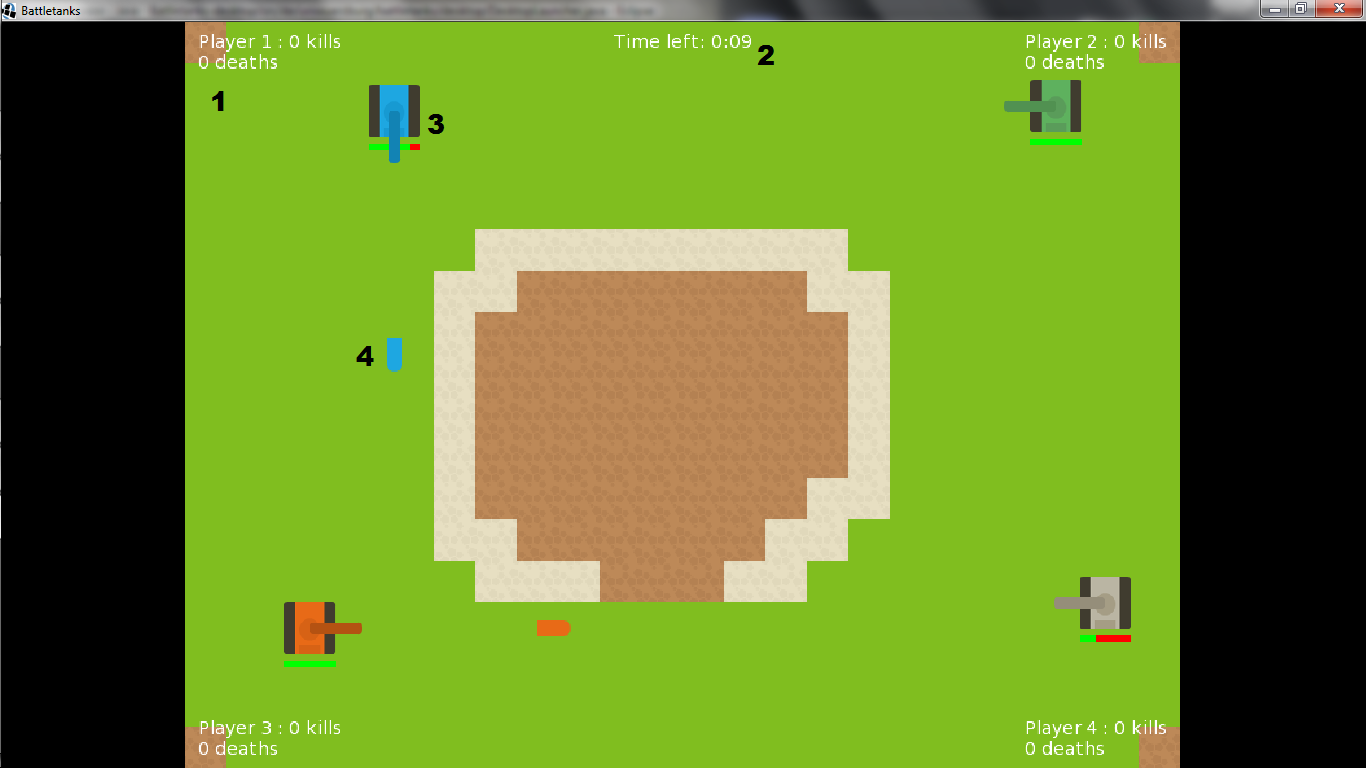
\includegraphics[width=15cm]{screenshot_game.png}    \caption{1: Anzeige von Abschüssen und Toden, 2: Verbleibende Spielzeit, 3: Panzer (Geschütz nach unten ausgerichtet), 4: Projektil des blauen Panzers}
\end{figure}



In den vier Ecken des Spielfelds werden die Anzahlen der Kills/Abschüsse sowie die Tode des jeweiligen Spielers angezeigt. (Abbildung 3: 1)
Die verbleibende Spielzeit sehen Sie oben in der Mitte des Spielfelds, wenn diese abgelaufen ist, ist das Spiel zu Ende und der EndScreen mit Scoreboard wird angezeigt. (Abbildung 3: 2)

Benutzen Sie die zugewiesene Tastenbelegung ihrer Spielfigur um ihre Figur zu bewegen sowie die Kanone ihrer Figur auszurichten. (Abbildung 3: 3) 

Mit Ihrer Schusstaste feuern Sie ein Projektil, welches sich in einer geraden Linie fortbewegt bis es auf ein Hindernis, den Spielfeldrand oder eine gegnerische Spielfigur trifft. (Abbildung 3: 4)

Falls das Projektil eine Spielfigur trifft wird der genommene Schaden auf der HP-Leiste der Figur angezeigt. Die übriggebliebenen Lebenspunkte werden als grüne Leiste angezeigt, fehlende als rote.
Wenn eine Spielfigur keine Lebenspunkte mehr besitzt erhöht sich die Anzahl der Tode des Spielers um 1. Die Abschüsse des Spielers, dessen Projektil den 'Todesstoß' ausgeführt hat, werden ebenfalls um 1 erhöht.

Der abgeschossene Spieler wird anschließend in der Spielfeldecke, die am weitesten von den anderen Spielfiguren entfernt ist 'wiederbelebt'.

\newpage
\subsection{Scoreboard}
\begin{figure}[H]
  \textbf{Screenshot Scoreboard:}\par\medskip
  \centering
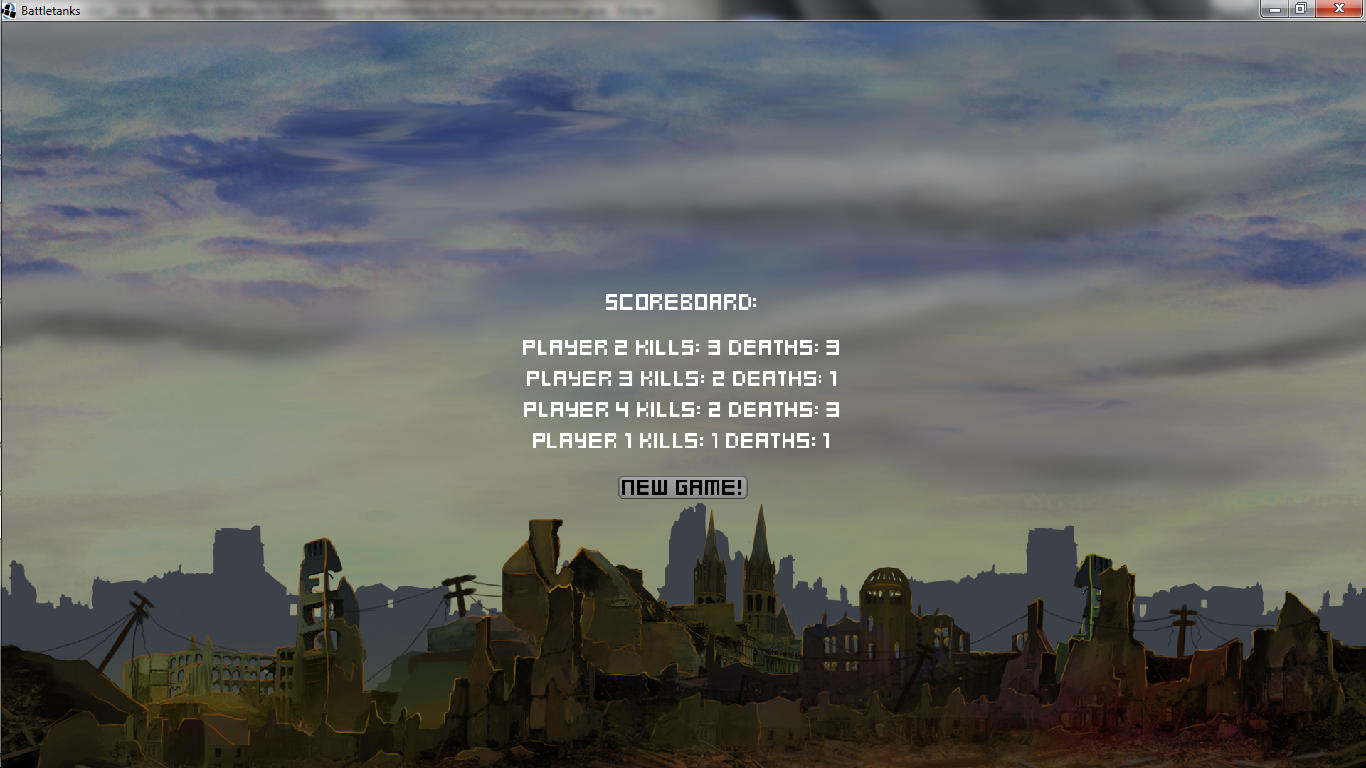
\includegraphics[width=15cm]{screenshot_endscreen.png}    
\caption{Spielende und Starten eines neuen Spiels}
\end{figure}


Das Scoreboard erscheint sobald die Spielzeit abgelaufen ist. Die Spieler werden nach der Anzahl ihrer Abschüsse und Tode sortiert. Bei gleich hoher Abschussanzahl zählt die geringere Anzahl an Toden, falls beide Werte gleich sind werden die Spieler nach Spielernummer sortiert.

Falls Sie eine weitere Partie spielen wollen drücken Sie nun auf den 'New Game'-Button, der das Menü wieder öffnet.





\end{document}